\section{Phase 1: Selecting Suitable Emotion Recognition Models}\label{sec:res-phase1}
In Phase 1, we mainly focused on evaluating how well different models performed when detecting emotional states using facial and vocal data. The evaluation was based on both the accuracy of emotion classification and how close the predicted intensity was to the acted intensity levels.


\subsection{Facial Expression Experiment}
This subsection discusses the results from the facial expression experiment. The emotion categorization performance of the models can be seen in Figure~\ref{fig:facial-category}, and the intensity identification results are shown in Figure~\ref{fig:facial-intensity}. In this experiment, two models were used: the HUME image expression model and CAGE.

\begin{figure}[H]
    \centering
    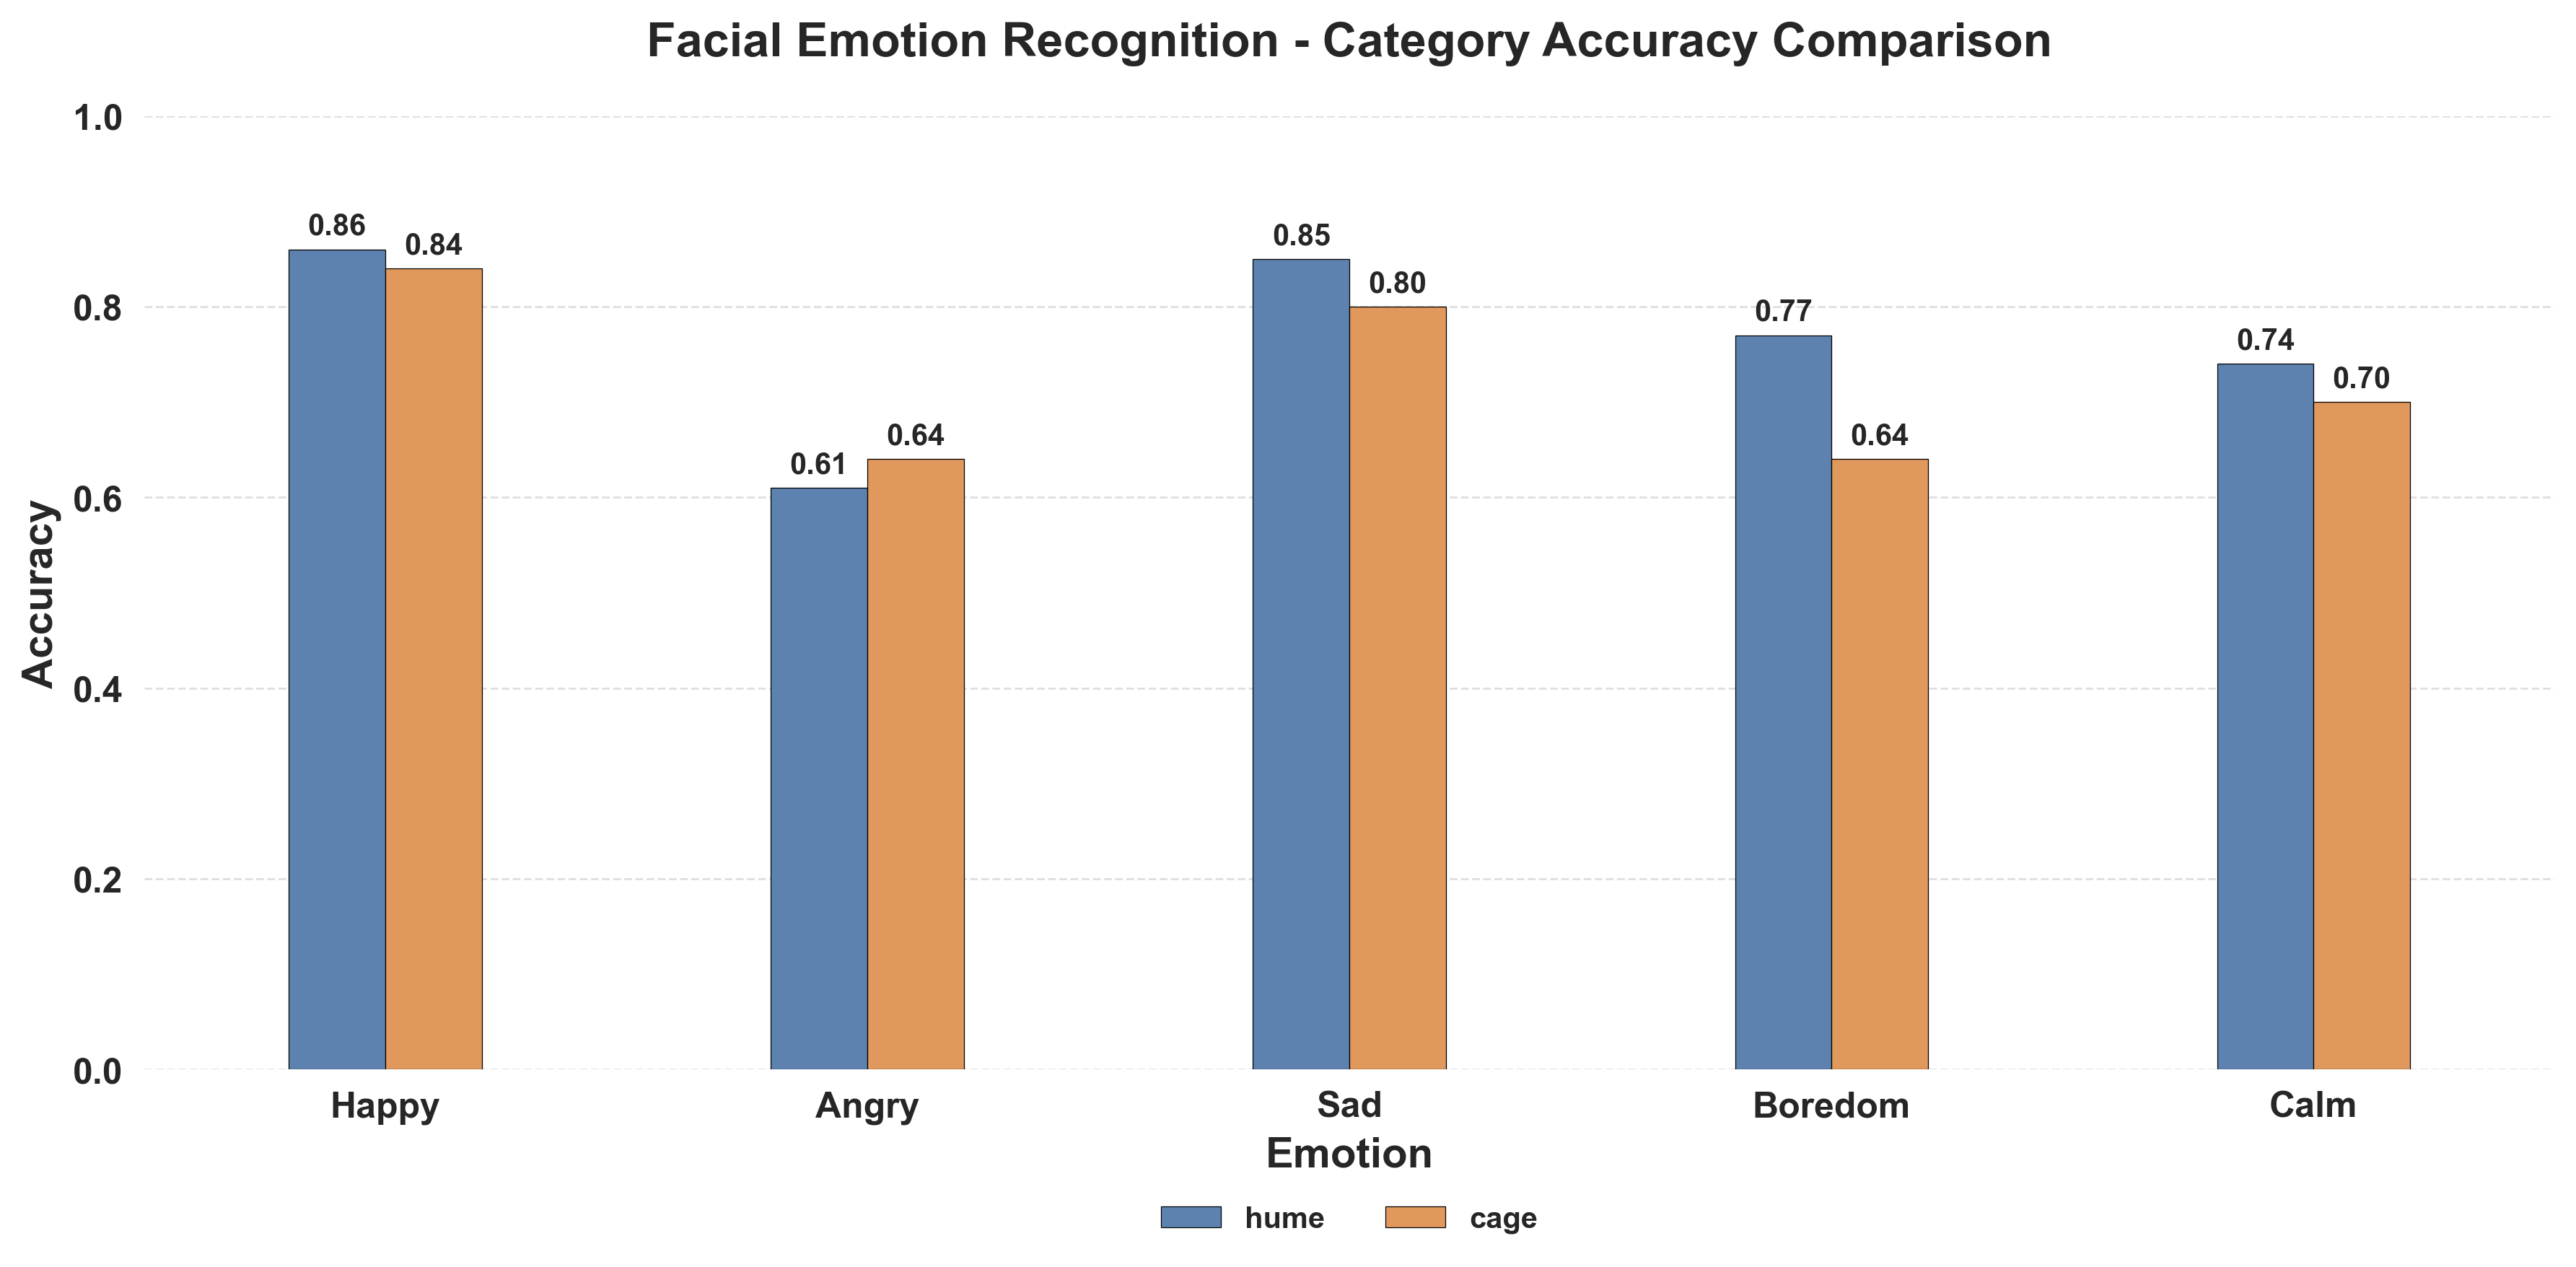
\includegraphics[width=1\textwidth]{img/chapter_04/facial_category_comparison}
    \caption{Emotion categorization results for facial expression experiment}
    \label{fig:facial-category}
\end{figure}

\begin{figure}[H]
    \centering
    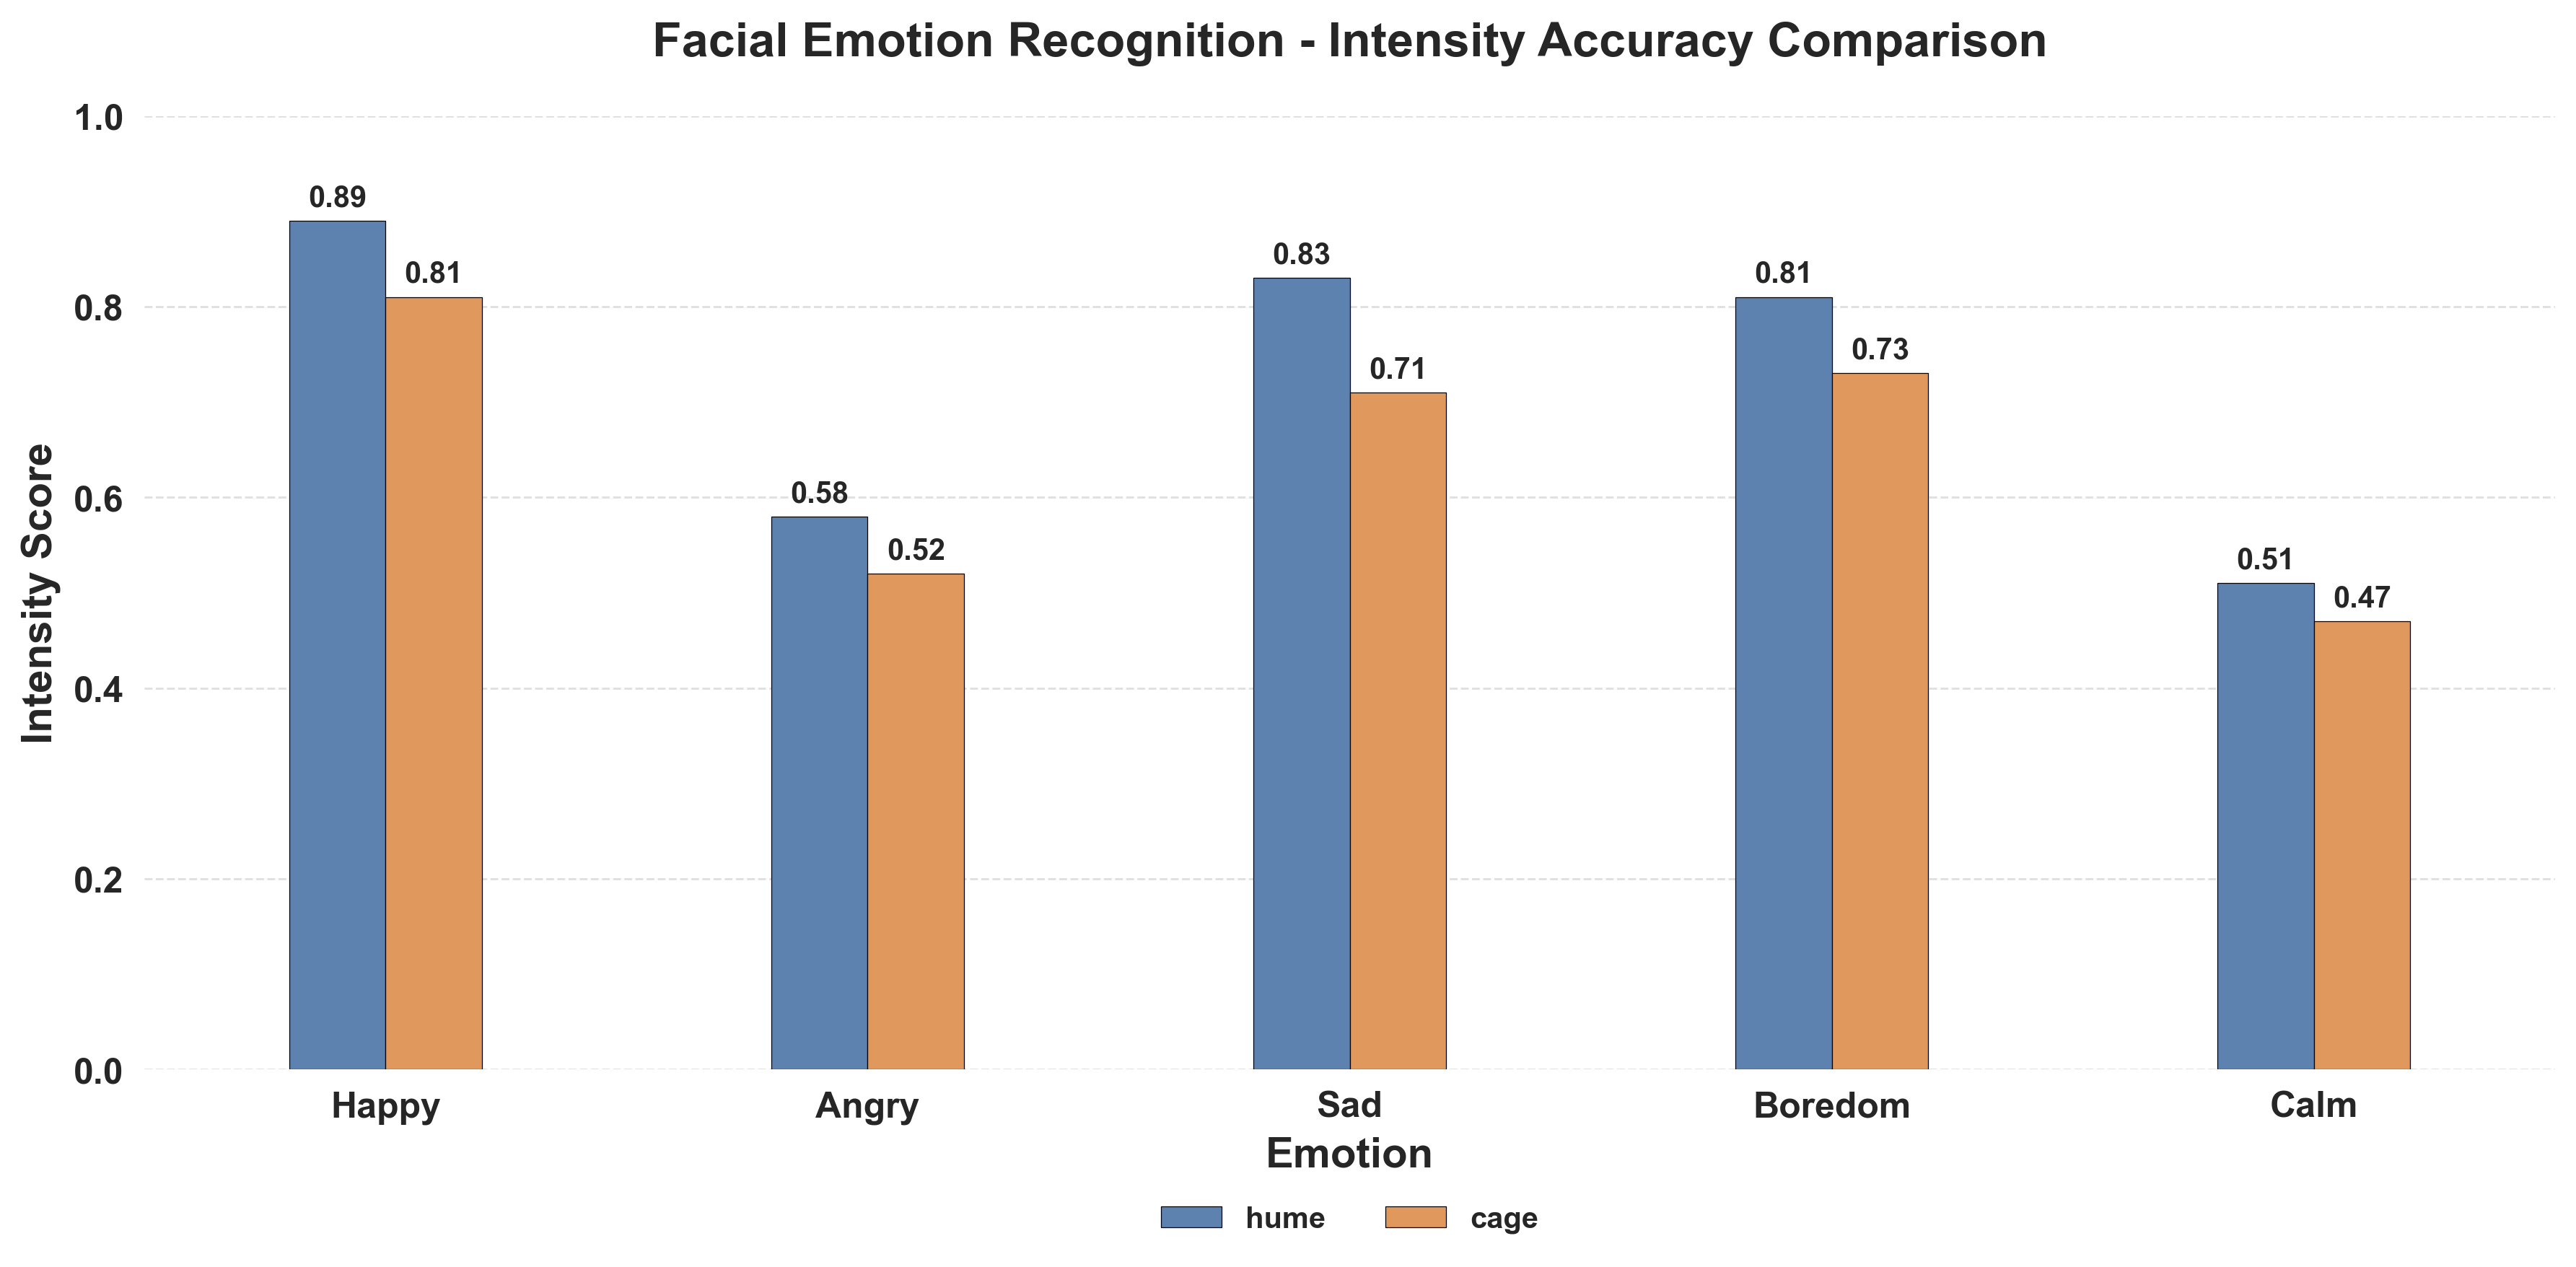
\includegraphics[width=1\textwidth]{img/chapter_04/facial_intensity_comparison}
    \caption{Emotion intensity identification results for facial expression experiment}
    \label{fig:facial-intensity}
\end{figure}

\subsubsection*{Observation}

This section presents a structured comparison of the performance of the CAGE and HUME models in emotion category recognition and intensity measurement, based on experimental results.

\paragraph*{Emotion Category Recognition}
Both models demonstrated high accuracy in detecting certain emotions, with varying performance across categories:
\begin{itemize}
    \item \textbf{Happy}: HUME achieved 86\% accuracy, slightly outperforming CAGE at 84\%.
    \item \textbf{Sad}: HUME recorded 85\% accuracy, compared to CAGE’s 80\%, showing a modest advantage.
    \item \textbf{Angry}: Both models struggled with anger recognition. CAGE performed slightly better at 64\%, compared to HUME’s 61\%. This difficulty may stem from participants struggling to express anger naturally during the experiment.
    \item \textbf{Boredom}: HUME outperformed CAGE, with 77\% accuracy compared to CAGE’s 64\%.
    \item \textbf{Calm}: HUME achieved 74\% accuracy, while CAGE recorded 70\%, indicating a slight edge for HUME.
\end{itemize}

\paragraph*{Intensity Measurement}
HUME generally outperformed CAGE in measuring emotion intensity across all emotions:
\begin{itemize}
    \item \textbf{Happy}: HUME achieved 89\% accuracy in intensity prediction, compared to CAGE’s 81\%.
    \item \textbf{Sad}: HUME recorded 83\% accuracy, significantly outperforming CAGE’s 71\%.
    \item \textbf{Angry}: HUME achieved 58\% accuracy, compared to CAGE’s 52\%, showing a modest improvement.
    \item \textbf{Boredom}: HUME outperformed CAGE, with 81\% accuracy compared to CAGE’s 73\%.
    \item \textbf{Calm}: HUME recorded 51\% accuracy, compared to CAGE’s 47\%. Both models struggled, often confusing high calmness with low boredom.
\end{itemize}

Both models performed well in detecting happiness and sadness, with HUME showing a slight edge in category recognition for most emotions. Anger recognition remained challenging for both, likely due to unnatural expressions by participants. HUME consistently outperformed CAGE in intensity measurement across all emotions, with particularly strong performance for happiness and sadness. The confusion between high calmness and low boredom suggests potential limitations in distinguishing subtle emotional states.


\subsection{Vocal Emotion Recognition Models Analysis}
This subsection presents the analysis of vocal emotion recognition experiments. The comparison was done between the HUME audio expression model and Wave2Vec2 model for both emotion category recognition and intensity identification. The results are shown in Figure~\ref{fig:vocal-category} and Figure~\ref{fig:vocal-intensity}.


\begin{figure}[H]
    \centering
    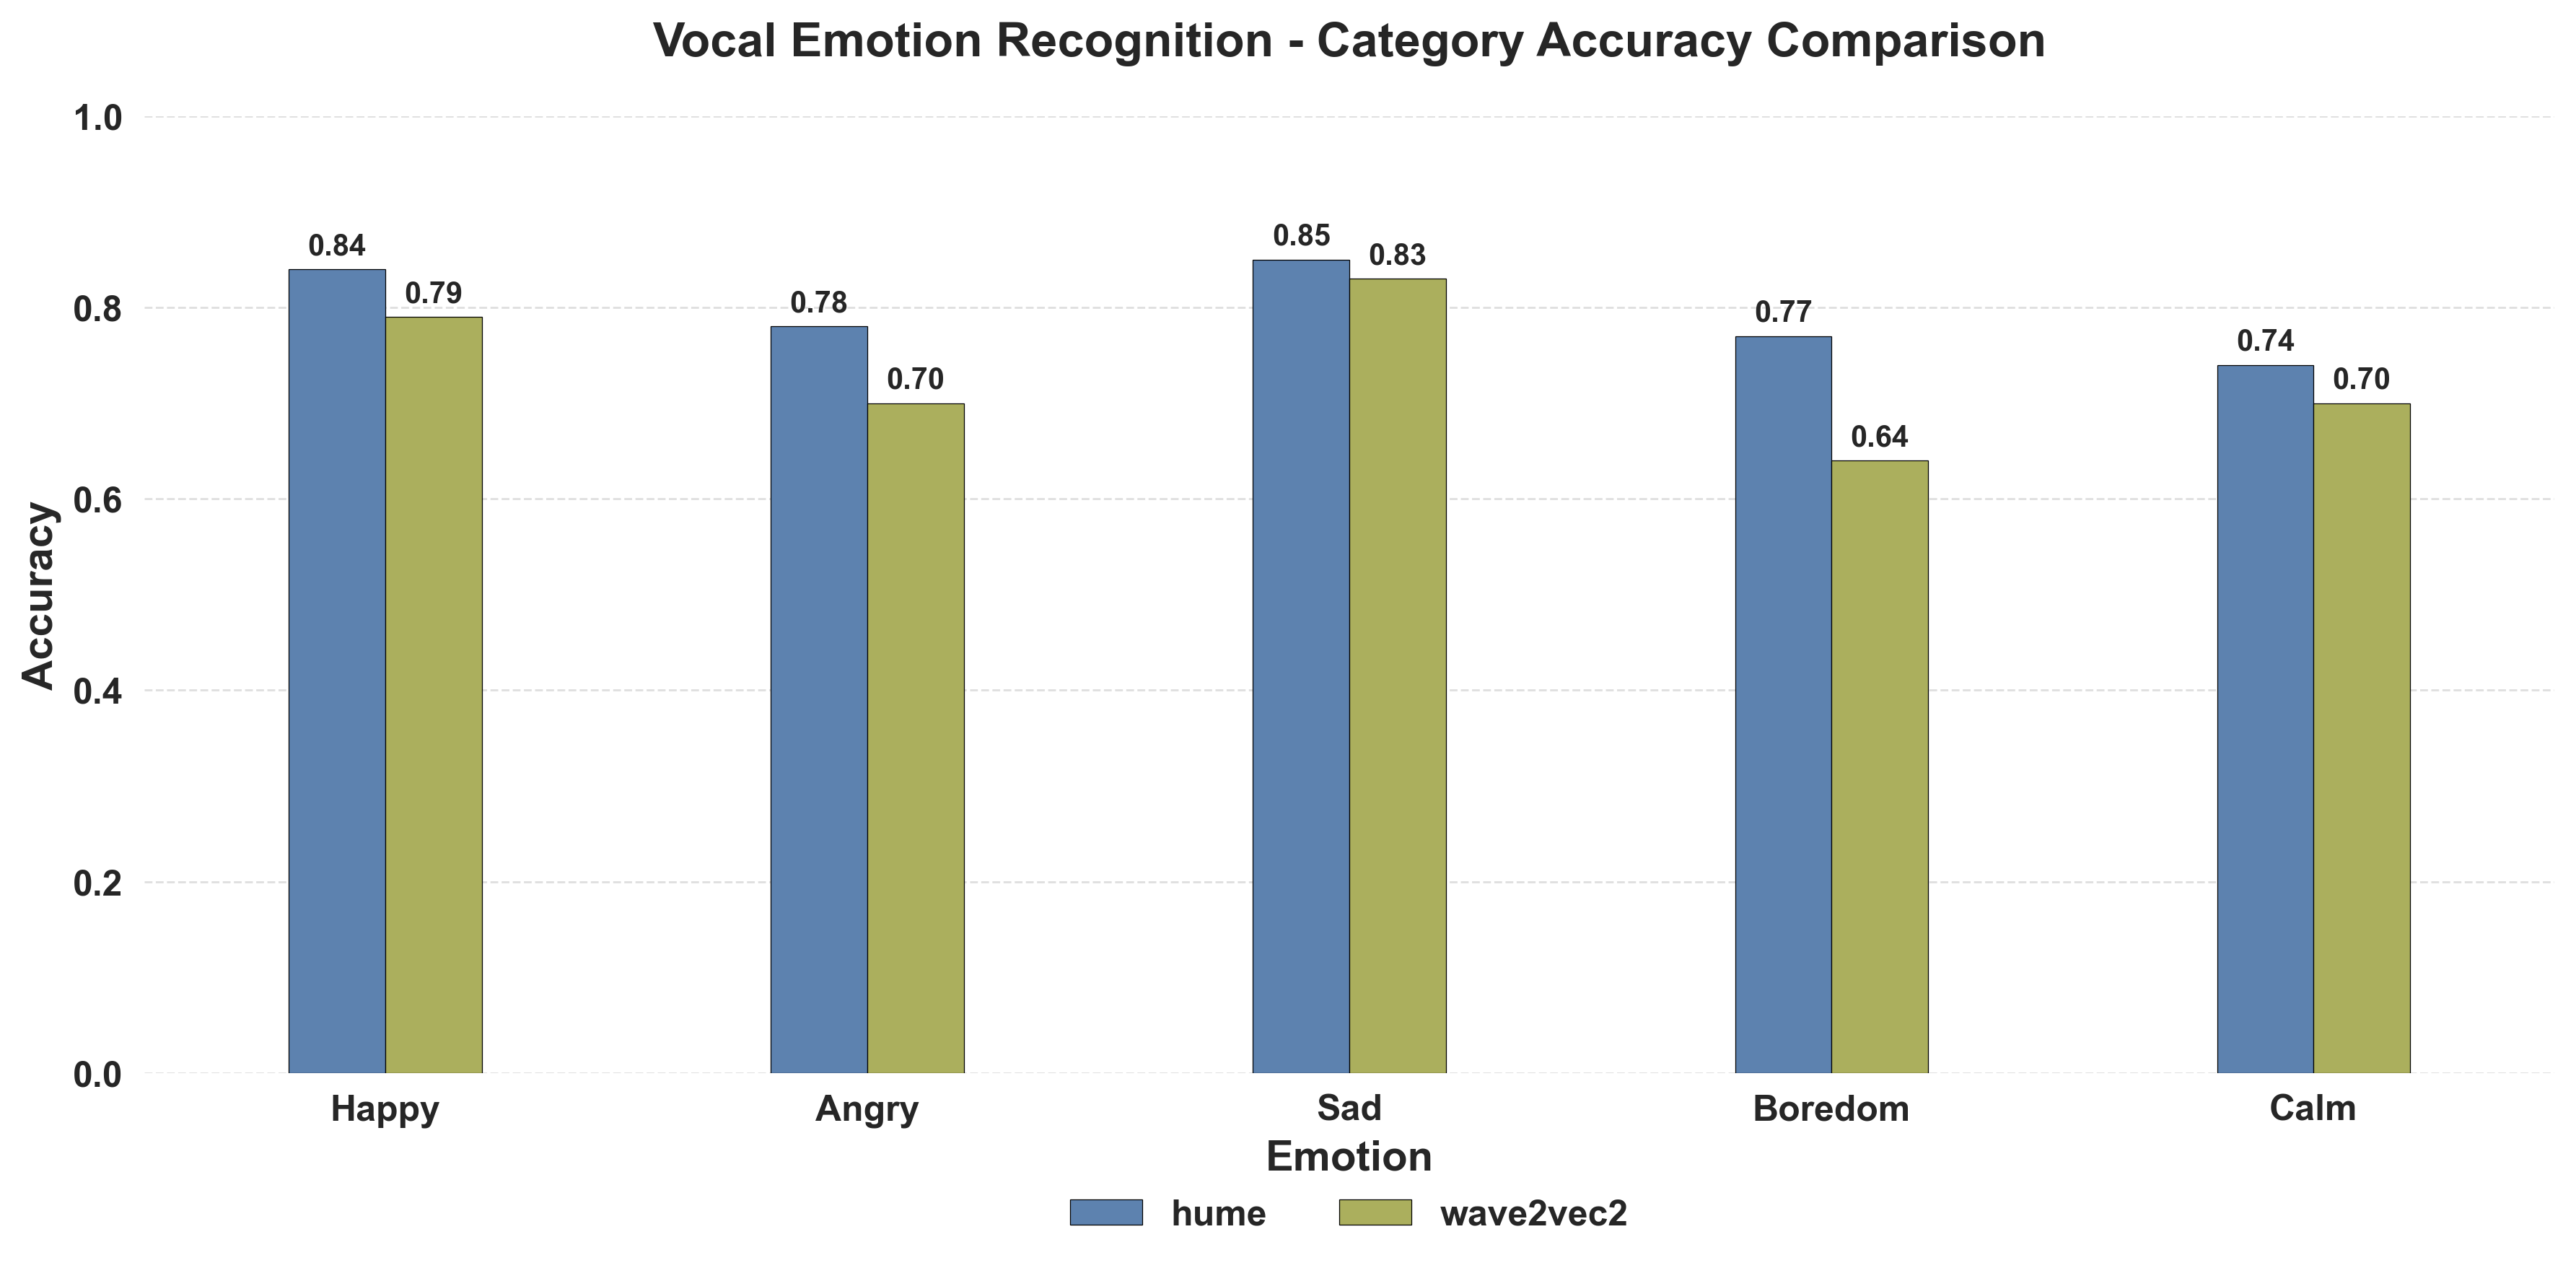
\includegraphics[width=1\textwidth]{img/chapter_04/vocal_category_comparison}
    \caption{Vocal emotion categorization results: HUME vs Wave2Vec2}
    \label{fig:vocal-category}
\end{figure}

\begin{figure}[H]
    \centering
    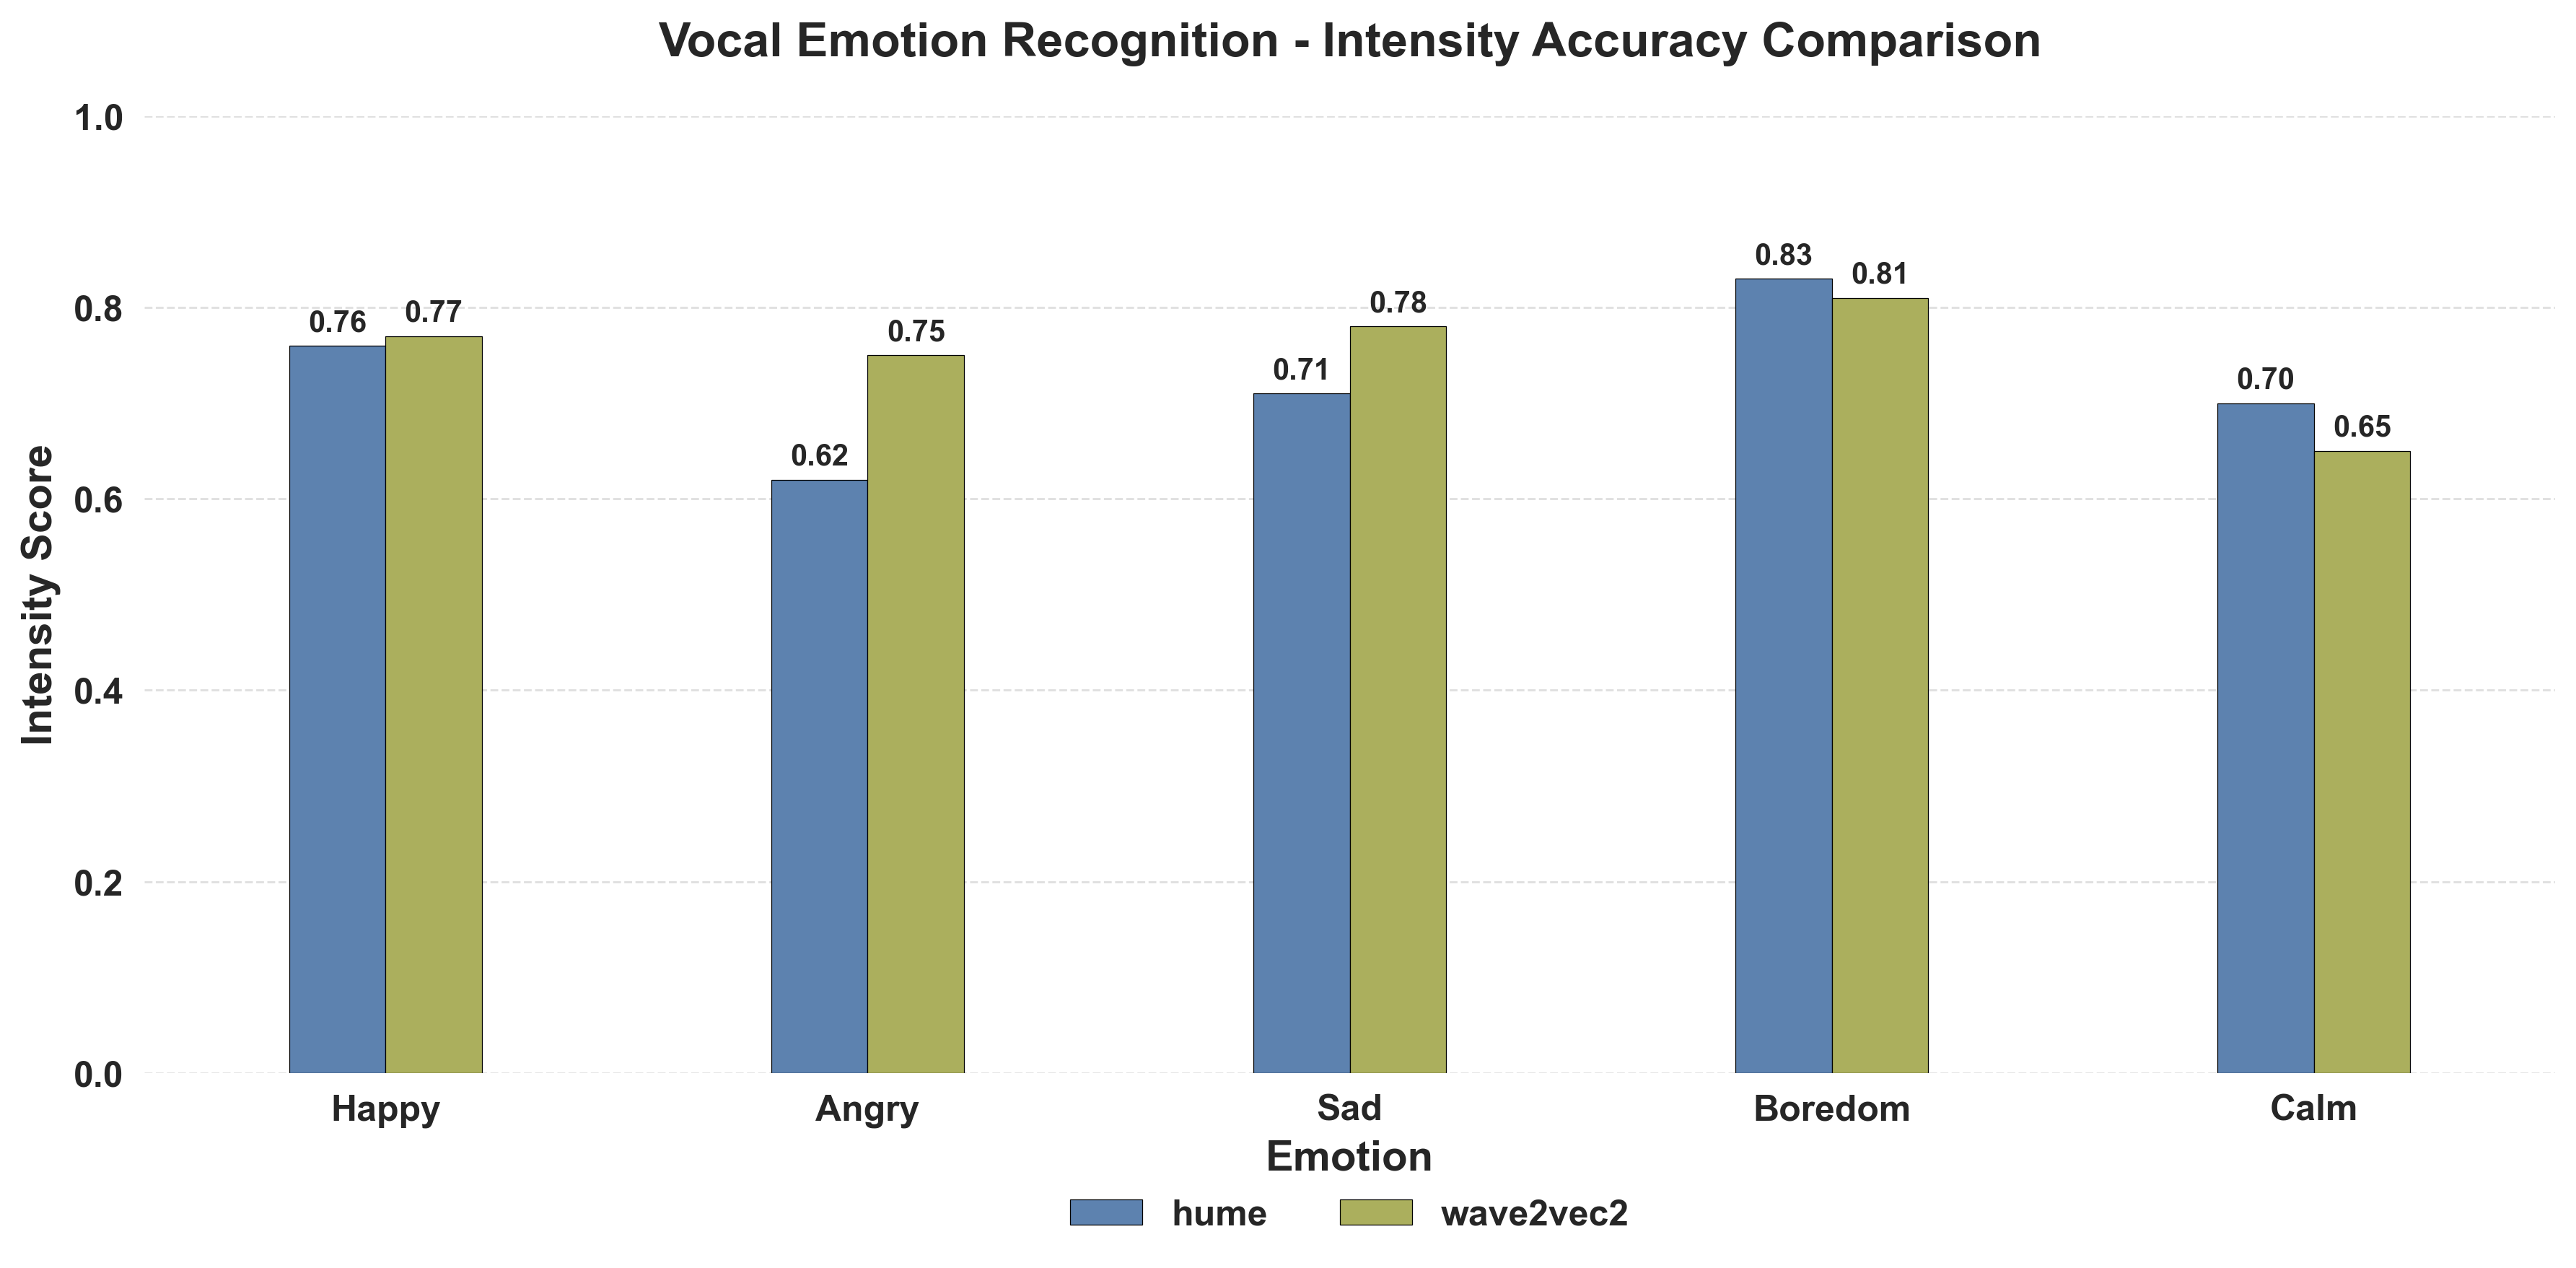
\includegraphics[width=1\textwidth]{img/chapter_04/vocal_intensity_comparison}
    \caption{Vocal emotion intensity identification: HUME vs Wave2Vec2}
    \label{fig:vocal-intensity}
\end{figure}


\subsubsection*{Observation}

This section presents a structured comparison of the performance of the HUME and Wave2Vec2 models in emotion category recognition and intensity measurement, based on experimental results for vocal data.

\paragraph*{Emotion Category Recognition}
Both models demonstrated varying performance across emotion categories:
\begin{itemize}
    \item \textbf{Happy}: HUME achieved 84\% accuracy, outperforming Wave2Vec2 at 79\%.
    \item \textbf{Sad}: Both models recognized sadness well, with HUME scoring 85\% and Wave2Vec2 83\%, showing a slight advantage for HUME.
    \item \textbf{Angry}: HUME performed better in category identification with 78\% accuracy, compared to Wave2Vec2’s 70\%.
    \item \textbf{Boredom}: HUME had stronger category recognition at 77\%, compared to Wave2Vec2’s 64\%.
    \item \textbf{Calm}: Both models had similar results, with HUME scoring 74\% and Wave2Vec2 70\%.
\end{itemize}

\paragraph*{Intensity Measurement}
Performance in measuring emotion intensity varied, with each model showing strengths for specific emotions:
\begin{itemize}
    \item \textbf{Happy}: Both models performed almost equally, with Wave2Vec2 achieving 77\% accuracy and HUME 76\%.
    \item \textbf{Sad}: Wave2Vec2 performed slightly better, with 78\% accuracy compared to HUME’s 71\%.
    \item \textbf{Angry}: Wave2Vec2 showed a clear advantage, achieving 75\% accuracy, compared to HUME’s 62\%.
    \item \textbf{Boredom}: Wave2Vec2 gave slightly better results, with 81\% accuracy compared to HUME’s 83\%.
    \item \textbf{Calm}: HUME was slightly better, with 70\% accuracy compared to Wave2Vec2’s 65\%.
\end{itemize}


Both models performed well in recognizing sadness, with HUME showing a slight edge in category recognition for most emotions, particularly happiness, anger, and boredom. Wave2Vec2 demonstrated strengths in intensity measurement, notably for anger and sadness, and performed comparably to HUME for happiness and boredom. The similar performance in calm category recognition suggests robustness in detecting subtler emotions, though intensity measurement differences indicate HUME’s slight advantage for calmness. These results highlight complementary strengths, with HUME excelling in category recognition and Wave2Vec2 in specific intensity measurements.

Based on these results, and since we are planning to perform a multimodal analysis in the next phase, we chose to continue with the HUME model to maintain consistency between the facial and vocal emotion recognition results.
